\documentclass{article}

\usepackage{graphicx}
\usepackage{rotating}
\usepackage{amsmath}
\usepackage{fancyhdr}
\usepackage{listings}
\usepackage{xcolor}
\usepackage{color}
\usepackage{textcomp}
\usepackage{float}
\usepackage[sorting=none]{biblatex}
\usepackage[margin=1in]{geometry}
\usepackage[font={small,it}]{caption}
\usepackage{placeins}
\usepackage{xepersian}

%\DeclareMathOperator*{\btie}{\bowtie}
\addbibresource{bibliography.bib}
\settextfont[Scale=1.2]{B-NAZANIN.TTF}
\setlatintextfont[Scale=1]{Times New Roman}
\renewcommand{\baselinestretch}{1.5}
\pagestyle{fancy}
\fancyhf{}
\rhead{تکلیف دوم درس مبانی بینایی کامپیوتر}
\lhead{\thepage}
\rfoot{علیرضا ابره فروش}
\lfoot{9816603}
\renewcommand{\headrulewidth}{1pt}
\renewcommand{\footrulewidth}{1pt}
%%%%%%%%%%
\lstset
{
    language=[latex]tex,
    basicstyle=\ttfamily,
    commentstyle=\color{black},
    columns=fullflexible,
    keepspaces=true,
    upquote=true,
    showstringspaces=false,
    morestring=[s]\\\%,
    stringstyle=\color{black},
}
%%%%%%%%%%
%beginMatlab
\definecolor{mygreen}{RGB}{28,172,0} % color values Red, Green, Blue
\definecolor{mylilas}{RGB}{170,55,241}
%endMatlab
\begin{document}
%beginMatlab
\lstset{language=Matlab,%
    %basicstyle=\color{red},
    breaklines=true,%
    morekeywords={matlab2tikz},
    keywordstyle=\color{blue},%
    morekeywords=[2]{1}, keywordstyle=[2]{\color{black}},
    identifierstyle=\color{black},%
    stringstyle=\color{mylilas},
    commentstyle=\color{mygreen},%
    showstringspaces=false,%without this there will be a symbol in the places where there is a space
    numbers=left,%
    numberstyle={\tiny \color{black}},% size of the numbers
    numbersep=9pt, % this defines how far the numbers are from the text
    emph=[1]{for,end,break},emphstyle=[1]\color{red}, %some words to emphasise
    %emph=[2]{word1,word2}, emphstyle=[2]{style},    
}
%endMatlab
\begin{titlepage}
\begin{center}

\includegraphics[width=0.4\textwidth]{figures/IUT Logo.png}\\
        
\LARGE
\textbf{دانشگاه صنعتی اصفهان}\\
\textbf{دانشکده مهندسی برق و کامپیوتر}\\
        
\vfill
        
\huge
\textbf{عنوان: تکلیف چهارم درس ریزپردازنده}\\
        
\vfill
        
\LARGE
\textbf{نام و نام خانوادگی: علیرضا ابره فروش}\\
\textbf{شماره دانشجویی: 9816603}\\
\textbf{نیم\,سال تحصیلی: پاییز 1400}\\
\textbf{مدرّس: دکتر عارف کریمی افشار}\\
\end{center}
\end{titlepage}


%\tableofcontents
\newpage


\section{}%1
ابتدا متغیرهای زیر را تعریف می‌کنیم.
\newline
$H$ و $W$: ابعاد تصویر
\newline
$I$: تصویر اصلی
\newline
$J$: تصویر مورد بررسی
\newline
$MAX_{I}$: بزرگ‌ترین سطح روشنایی محتمل در تصویر (مقدار پیش‌فرض 255)
\newline
$MIN_{I}$: کوچک‌ترین سطح روشنایی محتمل در تصویر (مقدار پیش‌فرض 0)

\subsection{\lr{MAE}}
\subsubsection{حداکثر}
حالتی را تصور می‌کنیم که اختلاف سطح روشنایی هر دو پیکسل متناظر در تصویر حداکثر باشد (تصویر تمام سیاه و تمام سفید). بنابراین به ازای هر $i$ و $j$ دامنه، $I(i, j)$ برابر $MAX_{I}$ و $J(i, j)$ برابر $MIN_{J}$ یا بالعکس. پس داریم:
\newline
\begin{latin}
$
\max(\frac{1}{H.W}\sum_{i=1}^{H}\sum_{j=1}^{W}\left| I(i, j) - J(i, j) \right|)=\frac{1}{H.W}\times H.W\times \left| MAX_{I} - MIN_{J} \right|=\left| MAX_{I} - MIN_{J} \right|
$
\end{latin}
که در حالت پیش‌فرض این مقدار برابر 255 است.
\subsubsection{حداقل}
حالتی را تصور می‌کنیم که اختلاف سطح روشنایی هر دو پیکسل متناظر در تصویر حداقل باشد (تصاویر برابر باشند). بنابراین به ازای هر $i$ و $j$ دامنه، $I(i, j)$ برابر $J(i, j)$ است. پس داریم:
\newline
\begin{latin}
$
\min(\frac{1}{H.W}\sum_{i=1}^{H}\sum_{j=1}^{W}\left| I(i, j) - J(i, j) \right|)=\frac{1}{H.W}\times H.W\times \left| I(i, j) - I(i, j) \right|=0
$
\end{latin}


\subsection{\lr{MSE}}
\subsubsection{حداکثر}
مشابه قسمت قبل، حالتی را تصور می‌کنیم که اختلاف سطح روشنایی هر دو پیکسل متناظر در تصویر حداکثر باشد (تصویر تمام سیاه و تمام سفید). بنابراین به ازای هر $i$ و $j$ دامنه، $I(i, j)$ برابر $MAX_{I}$ و $J(i, j)$ برابر $MIN_{J}$ یا بالعکس. پس داریم:
\newline
\begin{latin}
$
\max(\frac{1}{H.W}\sum_{i=1}^{H}\sum_{j=1}^{W} (I(i, j) - J(i, j))^{2})=\frac{1}{H.W}\times H.W\times (MAX_{I} - MIN_{J})^{2}=(MAX_{I} - MIN_{J})^{2}
$
\end{latin}
که در حالت پیش‌فرض این مقدار برابر 65025 است.
\subsubsection{حداقل}
مشابه قسمت قبل، حالتی را تصور می‌کنیم که اختلاف سطح روشنایی هر دو پیکسل متناظر در تصویر حداقل باشد (تصاویر برابر باشند). بنابراین به ازای هر $i$ و $j$ دامنه، $I(i, j)$ برابر $J(i, j)$ است. پس داریم:
\newline
\begin{latin}
$
\min(\frac{1}{H.W}\sum_{i=1}^{H}\sum_{j=1}^{W} (I(i, j) - J(i, j))^{2})=\frac{1}{H.W}\times H.W\times (I(i, j) - I(i, j))^{2}=0
$
\end{latin}


\subsection{\lr{PSNR}}
برای بیشینه (کمینه) کردن تابعِ 
$
10\log_{10}(\frac{MAX_{I}^{2}}{MSE})
$
کافیست تابعِ
$
\frac{MAX_{I}^{2}}{MSE}
$
بیشینه (کمینه) کنیم.
\subsubsection{حداکثر}
با فرض ناصفر بودن مقدار $MAX_{I}$ داریم:
\newline
\begin{latin}
$
\max(10\log_{10}(\frac{MAX_{I}^{2}}{MSE}))=\lim_{MSE \to 0 } (10\log_{10}(\frac{MAX_{I}^{2}}{MSE}))=\infty
$
\end{latin}
پس به ازای دو تصویر با \lr{MSE}ِ نزدیک به صفر (دو تصویر تقریبا برابر)، مقدار \lr{PSNR} به بی‌نهایت میل می‌کند.
\subsubsection{حداقل}
داریم:
\newline
\begin{latin}
$
\min(10\log_{10}(\frac{MAX_{I}^{2}}{MSE}))=10\log_{10}(\frac{MAX_{I}^{2}}{(MAX_{I}-MIN_{J})^{2}})
$
\end{latin}
که در حالت پیش‌فرض برابر است با:
\newline
\begin{latin}
$
10\log_{10}(\frac{255^{2}}{65025})=0
$
\end{latin}






\section{}%2
سطح روشنایی هر پیکسل در تصویر خاکستری‌گونه از $MIN_{I}$ (پیش‌فرض 0) تا $MAX_{I}$ (پیش‌فرض 255) متغیر است. بدترین \lr{MSE} که در واقع بزرگ‌ترین \lr{MSE} است زمانی رخ می‌دهد که اختلاف سطح روشنایی هر دو پیکسل متناظر در تصاویر ماکسیمم باشد. در نتیجه برای ساخت چنین تصویری فاصله‌ی سطح روشنایی هر پیکسل در تصویر اولیه را از مقادیر $MIN_{I}$ و $MAX_{I}$ به دست می‌آوریم (قدر مطلق تفاضل). در صورتی که سطح روشنایی به $MIN_{I}$ (سیاه) نزدیک‌تر بود، مقدار $MAX_{I}$ (سفید) و در صورتی که به $MAX_{I}$ (سفید) نزدیک‌تر بود، مقدار $MIN_{I}$ (سیاه) را در پیکسل متناظر قرار می‌دهیم. در این حالت چون قدر مطلق تفاضل‌ها به ازای همه پیکسل‌های تصویر ماکسیمم هستند پس تضمین می‌شود که ماکسیمم \lr{MSE}(بدترین \lr{MSE}) را نسبت به تصویر ورودی داریم.





\section{}%3
\subsection{الف}
\begin{latin}
\lstinputlisting{sources/p3a.m}
\end{latin}

\subsection{ب}
\begin{latin}
\lstinputlisting{sources/p3b.m}
\end{latin}

\subsection{ج}
\begin{latin}
\lstinputlisting{sources/p3c.m}
\end{latin}
با مقایسه‌ی \lr{PSNR} در دو تصویر تولید شده در قسمت‌های قبل درمی‌یابیم که بهتر بودن \lr{PSNR}ِ یک تصویر نسبت به تصویر دیگر الزاما به معنی بهتر بودن کیفیت بصری آن تصویر نیست. همانطور که می‌بینیم، تصویر تولید شده توسط الگوریتم \lr{Floyd-Steinberg} با وجود داشتن \lr{PSNR}ِ پایین‌تر نسبت به تصویر تولید شده توسط الگوریتم حریصانه (تابع \lr{toBlackWhite}) جزئیات تصویر را بهتر مشخص می‌کند و کیفیت بصری بهتری دارد. پس نتیجه می‌گیریم که \lr{PSNR} در همه جا معیار دقیقی برای مقایسه‌ی کیفیت تصاویر نیست.
\begin{figure}[H]
    \centering
    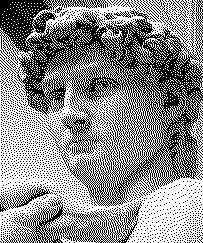
\includegraphics[width=0.25\textwidth]{figures/3c1.jpg}
    \caption
	{
خروجی الگوریتم \lr{Floyd-Steinberg}
	}
    \label{fig:fig1}
\end{figure}
\begin{figure}[H]
    \centering
    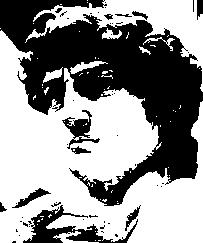
\includegraphics[width=0.25\textwidth]{figures/3c2.jpg}
    \caption
	{
خروجی الگوریتم حریصانه
	}
    \label{fig:fig1}
\end{figure}

%%%%%%%%%%%%%%%%%%%%%%%%%%%%%%%%%%%


%\begin{latin}
%\lstinputlisting{sources/p1.m}
%\end{latin}



%%%%%%%%%%%%%%%%%%%%%%%%%%%%%%%%%%%
%%%%%%%%%%%%%%%%%%%%%%%%%%%%%%%%%%%
%%%%%%%%%%%%%%%%%%%%%%%%%%%%%%%%%%%

%------------------------------------------------------------------------------------------


\section*{منابع}
\renewcommand{\section}[2]{}%
\begin{thebibliography}{99} % assumes less than 100 references
%چنانچه مرجع فارسی نیز داشته باشید باید دستور فوق را فعال کنید و مراجع فارسی خود را بعد از این دستور وارد کنید


\begin{LTRitems}

\resetlatinfont

\bibitem{b1}
\end{LTRitems}

\end{thebibliography}


\end{document}
